\documentclass[a4paper,11pt]{scrartcl}

\usepackage[ngerman]{babel} 
\usepackage[T1]{fontenc}
\usepackage[utf8]{inputenc}
\usepackage{hyperref}

\usepackage{amsmath,amsfonts,amssymb}
\usepackage{graphicx}
\usepackage{siunitx}

\usepackage{epstopdf}

\setcounter{section}{4}


\begin{document}
\hfill Alexander Schnapp

\hfill Max Menges

\begin{center}
\underline{\Huge{Intro HPC: Blatt 4}}\\
\large{17.11.1014}\\
\end{center}

\subsection{Reading}

\subsection{Matrix Multiply -- parallel version using MPI}
For the Matrix Multiply in parallel version we use the source code 'matrix\_ multiply.cc'. To run and compile use our file 'make+run.sh'.

In this code we first initialise the matrizes A and B by the master process (rank==0). This process is then distributing the diffrent lines of A to the different slave processes. The Matrix B is distributet to all processes completely.
After the processes have calculated the result resulting of a line of A they are sending the result back to the master process.
After this has got all the results it prints the solution. (This is not contribution to the calculation time). 

The outcome of this calculation is the following Matrix C:

\begin{tabular}{|c|c|c|c|c|}
\hline 
0 & 30 & 60 & 90 & 120 \\ 
\hline 
0 & 40 & 80 & 120 & 160 \\ 
\hline 
0 & 50 & 100 & 150 & 200 \\ 
\hline 
0 & 60 & 120 & 180 & 240 \\ 
\hline 
0 & 70 & 140 & 210 & 280 \\ 
\hline 
\end{tabular} 



\subsection{Matrix Multiply -- scaling process count}

We now excecute our programm with a diffrent number of processes. For that we encount the nodes creek[01-04]. We are calculation a Matrix of 1000x1000 entries. This wwe compare with our sequential implementation.

Plotting the Time that was needed for the calculations we see that its decreasing very fast but is reaching limit very soon.

\begin{figure}[!h]
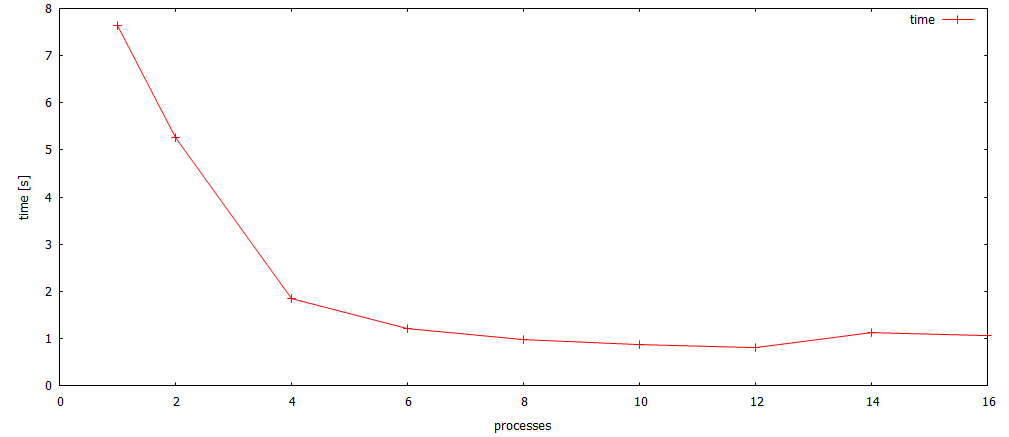
\includegraphics[width=\linewidth,
keepaspectratio]{2_3a}
\centering

\end{figure}

Plotting the speed-up we see a increase very similar to a linear speed up in the beginnen but then it starts to deviate more and more.
\begin{figure}[htbp]
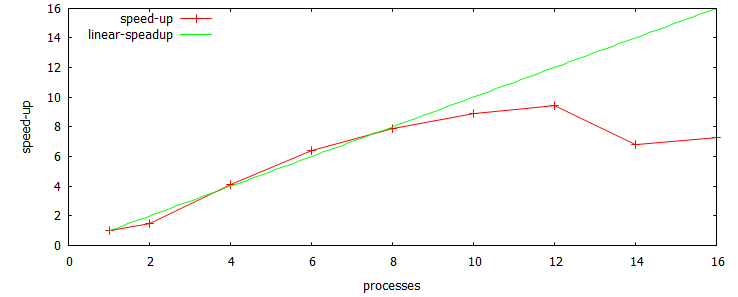
\includegraphics[width=\linewidth,
keepaspectratio]{2_3b}
\centering

\end{figure}

The Effeciency is nearly 1 for about 4-8 processes but then drastically decreasing for higher numbers.

\begin{figure}[htbp]
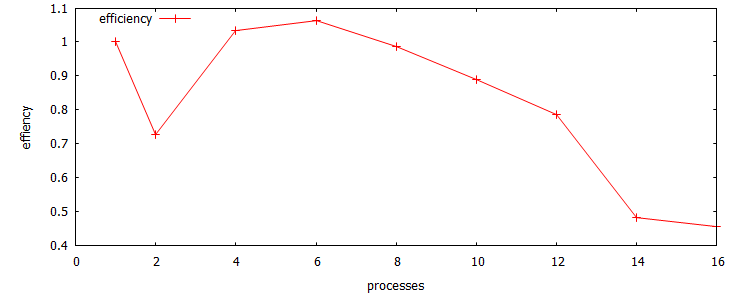
\includegraphics[width=\linewidth,
keepaspectratio]{2_3c}
\centering

\end{figure}

All this is a consequence of the process and the used data being at is best at about 4-8 processes. With higher values the message traffic gets too high, so that the parallalization is not very effective any more. 
\subsection{Matrix Multiply -- scaling problem size}
This can be changed if you have more data, so that the single process is having more work to do with nearly the same ammount of messege traffic.

\end{document}
